%---------- Primeiro Capitulo ----------
\chapter{Introdução}
\label{chap:intro}

O propeller clock depende de um fenômeno chamado \sigla{POV}{Persistência da visão} (Persistence of vision, em inglês). Persistência da visão consiste no fenômeno observado quando um objeto visto pelo olho humano persiste na retina por uma fração de segundo após a sua percepção. Assim, imagens projetadas com uma frequência superior a 16Hz associam-se na retina sem interrupção~\cite{Wikipedia2013}~\cite{Anderson1993}.

Segundo essa teoria, ao captar uma imagem, o olho humano levaria uma fração de tempo para "apagá-la". Assim, quando os quadros de um filme de cinema são projetados na tela, o olho mistura o quadro anterior com o seguinte, provocando a ilusão de movimento: um objeto colocado à esquerda num quadro, aparecendo à direita no quadro seguinte, cria a ilusão de que o objeto se desloca da esquerda para a direita.

Posteriormente foi comprovado que este fenômeno é mais complexo, e melhor explicado quando divido entre Movimento \simbolo{$\phi$}{Phi} e Movimento \simbolo{$\beta$}{Beta}, pelo psicólogo checo Max Wertheimer. Porém esta análise fisiológica da visão foge do escopo desse trabalho~\cite{Kaufman1974}.

A persistência da visão pode ser observada no cotidiano ao se ligar um ventilador. Assim que o ventilador acelera, não é possível ver as hélices individualmente, somente um círculo.

Isso se aplica ao nosso trabalho pois ao rotacionar rapidamente uma hélice com diversos \sigla{LED}{Diodo emissor de luz}s, e ao coordenar o acendimento dos mesmos, é possível produzir imagens claramente visíveis ao olho humano.

\section{Componentes} %GEANINE
%Lista dos componentes utilizados e custo aproximado de cada um
A tabela 1 mostra uma relação dos materiais necessários para a confecção do display de varredura mecânica.

\begin{table}[!h]
	\centering
	\label{tab:lista-materiais-propeller}
	\begin{tabular}{ccc}
		\hline
		Produto & Quantidade & Valor (Individual) \\
		\hline
		Arduino Nano & 1 & R\$44,00 \\
		Latch 74LS373 & 1 & R\$1,85 \\
	    Regulador de tensão 5V - 7805 & 1 & R\$1,00 \\
		Capacitor 47\simbolo{$\mu$}{micro}F & 1 & R\$0,75 \\
        Cristal 40MHz & 1 & R\$0,70 \\
        Matriz de Resistores 330{$\Omega$} & 2 & R\$0,08 \\
        LED RGB & 16 & R\$1,10 \\
        Barra de Pinos 28 pinos & 1 & R\$0,60 \\
        Barra de Pinos 20 pinos & 2 & R\$0,60 \\
        Diodo emissor IR & 1 & R\$0,80 \\
        Fototransistor & 1 & R\$0,80 \\
        Barra de pinos 30 pinos & 1 & R\$0,60 \\
        Matriz de Contatos de Cobre & 1 & R\$8,90 \\
        Cooler 3800 RPM & 1 & R\$9,10 \\
        Slot Bateria 9V & 1 & R\$---- \\
        Total & - & R\$88.06 \\
		\hline
	\end{tabular}
    \caption[Orçamento para o Display de Varredura Mecânica]{Orçamento para o Display de Varredura Mecânica}
\end{table}


Além do desenvolvimento do display de varredura mecânica, foi necessário desenvolver um Tacômetro digital para Arduino, para ser possível testar a frequência do Cooler utilizado no projeto. Entretanto, este dispositivo será apenas utilizado como ferramenta de desenvolvimento, não fazendo parte da versão final do mesmo.

A lista de materiais para este projeto está listada na tabela 2:

\begin{table}[!h]
	\centering
	\label{tab:lista-materiais-tacometro}
	\begin{tabular}{ccc}
		\hline
		Produto & Quantidade & Valor (Individual) \\
		\hline
		Arduino Nano & 1 & R\$44,00 \\
	    Trimpot 5k\simbolo{$\Omega$}{Omega} & 1 & R\$0,58 \\
        Barra de pinos 30 pinos & 1 & R\$0,60 \\
        Transistor NPN 2n2222 & 2 & R\$0,25 \\
        LED IR & 1 & R\$0,80 \\
        Fototransistor & 1 & R\$0,80 \\
        Resistor 10{$\Omega$} & 1 & R\$0,08 \\
        Resistor 100k{$\Omega$} & 1 & R\$0,08 \\
        Resistor 15k{$\Omega$} & 1 & R\$0,08 \\
        Protoboard & 1 & R\$86,90 \\
        Total & - & R\$134,42 \\
		\hline
	\end{tabular}
    \caption[Lista de materiais utilizados no Tacômetro Digital]{Lista de materiais utilizados no Tacômetro Digital}
\end{table}

%b) "Quais partes constituem o dispositivo e como interagem entre si?" (utilizar um diagrama de blocos como auxiliar na descrição)
Uma breve descrição dos principais componentes que constituem o projeto será realizada neste momento:

\begin{itemize}
\item Arduino Nano: Será utilizado para realizar todo o processamento de informações necessário no projeto, como por exemplo, o cálculo do número de rotações da hélice, o controle dos LEDs, entre outros.
\item Latch 74LS373: Circuito integrado responsável por controlar o acendimento dos LEDs. Este componente é necessário devido ao baixo número de portas de saída por parte do Arduino.
\item Regulador de tensão 5V – 7805: O regulador de tensão é necessário para poder limitar a tensão nos LEDs, pois a diferença de potencial necessária nestes componentes é menor do que é necessário no cooler.
\item Capacitor 47 {$\mu$}F: Utilizado como filtro no regulador de tensão.
\item Cristal 40MHz: Utilizado para contar o tempo corretamente no relógio.
\item Matriz de Resistores 330{$\Omega$}: Utilizada para regular a corrente que vai para os LEDs
\item LED RGB: Utilizados para criar o efeito de ilusão de óptica ao acenderem nos momentos certos.
\item Socket 28 pinos: Utilizados para poder fixar o Arduino na matriz de contato.
\item Diodo emissor IR e Fototransistor: Utilizados para realizar a contagem de rotações por minuto do cooler.
\item Cooler 3800 RPM: Melhor escolha para o motor pois já possui um circuito pronto de potência e velocidade. Deve ser de no mínimo 3600 rpm para criar um bom efeito visual.
\end{itemize}

\section{Conteúdos Envolvidos} %LEONARDO

Para o desenvolvimento deste projeto, diversos são os conhecimentos necessários envolvendo diferentes áreas, desde eletrônica e programação até a física envolvida por trás de alguns aspectos da visão.

Na área de eletrônica, é necessário compreender os seguintes aspectos:
\begin{itemize}
\item Sensores IR: Existem sensores de infravermelho ativos e passivos. Um sensor de infravermelho ativo é composto por um emissor de luz infravermelha e um receptor, que reage a essa luz. Por sua vez, um sensor de infravermelho passivo não emite luz infravermelha, mas apenas capta esse tipo de luz no ambiente~\cite{RoboLivre2014}.

    Neste projeto, usaremos sensores de infravermelho para medir as rotações do relógio.
\item Construção da \sigla{PCI}{Placa de Circuito Impresso}: Será necessária a contrução de uma placa de circuito impresso para o projeto. Nela estarão contidos, entre outros componentes, os LEDs, posicionados da maneira correta para a visualização otimizada da saída do projeto. É necessária a compreensão de todos os passos para a criação da matriz.
\end{itemize}

Na área de programação, é fundamental compreender como programar o Arduino, pois é ele quem controla o acendimento dos LED's~\cite{Arduino2014}~\cite{ArduinoRef2014}.

Na área de mecânica é imprescindível o cálculo exato das rotações do motor. Erros, mesmo que pequenos, nesta etapa são suficientes para que a imagem final seja diferente do esperado.

Entretanto, a principal preocupação será com conceitos de POV e cadência, uma vez que abrangem a parte principal do projeto: o objetivo de causar uma ilusão aos olhos do espectador para criar uma imagem~\cite{Anderson1993}.

	O projeto também envolve conhecimento na área de eletrônica e programação, é preciso desenvolver hardware e software que apliquem corretamente os conceitos teóricos estudados. O primeiro projeto similar desenvolvido foi feito em 1995 por Bob Blick e será utilizado como referência para o desenvolvimento deste trabalho~\cite{Blick2002}.

\section{Metodologia de Execução} %TODOS JUNTOS

%a) Quais são as tarefas *específicas'* necessárias para a execução do projeto? Descrever brevemente o que envolve cada tarefa.
%b) Quais as relações de dependência entre as tarefas?
%c) Quanto tempo está previsto para cada tarefa (estimativa)?
%Sugestão: utilizar um diagrama Gantt

Será necessário construir peças, realizar testes e desenvolver o software do projeto. Construiremos um tacômetro, um motor para rotacionar a placa e uma matriz de contatos.
A construção do motor depende da construção do tacômetro, enquanto o desenvolvimento do software depende de toda a parte de hardware estar pronta pois testes são fundamentais durante o processo de desenvolvimento.

A duração de cada tarefa varia, com algumas durando apenas um dia e outras mais de uma semana. A tarefa que mais levará tempo é a redação da monografia, pois será feita com o decorrer do projeto.

O diagrama de blocos, utilizado para demonstrar de forma simples a relação entre cada componente do projeto, está mostrado na Figura 1.

\begin{figure}[!h]
	\centering
	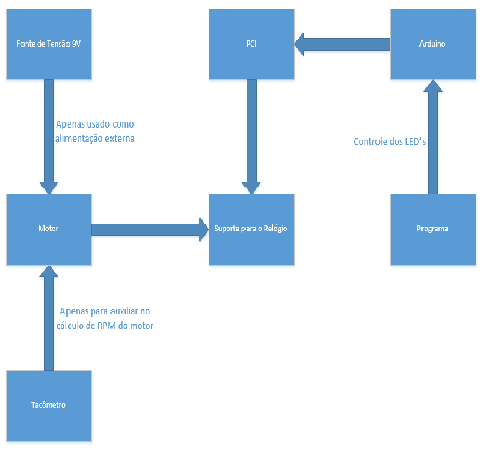
\includegraphics{./Diagrama_Blocos.png}
	\caption[Diagrama de Blocos do projeto]{Diagrama de Blocos do projeto}
	\label{fig:Diagrama_Blocos}
\end{figure}

\begin{itemize}
\item Construção do tacômetro:
Serão usados um LED infravermelho e um receptor infravermelho, além do cooler onde serão posicionados. Com esse sistema é possível contar quantas vezes o sinal é cortado pelas hélices do cooler, e assim podemos calcular o número de rotações por minuto do sistema. Os cálculos serão efetuados com um arduino.
\item Construção da matriz de contatos:
São duas etapas, o design e a construção. No design será desenhado como a placa será impressa e onde irão os componentes. Na construção, produziremos a placa com peróxido e depois soldaremos os componentes nela.
\item Construção do motor:
Para construir o motor, as hélices do motor serão removidas e o motor será fixado em uma base com uma fonte de alimentação.
\item Integração das peças de hardware:
Para poder prosseguir com o projeto e finalizar o hardware, a matriz de contatos, o motor e o Arduino serão integrados.
\item Desenvolvimento do software:
Será desenvolvido um algoritmo que coordene o acender e apagar dos LEDs para que, ao girarem, formarão uma imagem. O arduino será programado. Para programar, usaremos uma interface no computador que nos permite programar em C e passar esse código para o arduino através da uma porta USB.
\end{itemize}

O diagrama de Gantt do projeto, com as principais tarefas especificadas, está mostrado na figura 2.

\begin{figure}[!h]
	\centering
	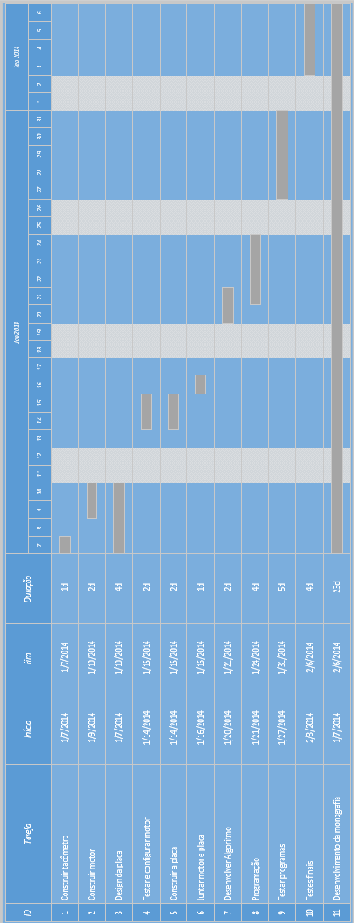
\includegraphics{./Diagrama_Gantt.png}
	\caption[Diagrama de Gantt do projeto]{Diagrama de Gantt do projeto}
	\label{fig:Diagrama_Gantt}
\end{figure}

\section{Banca Examinadora}
\begin{itemize}
\item Aluno convidado:
Iuri Barcat
\item Professor Orientador:
César Benitez (DAELN)
\item Professora convidada:
Leyza Dorini (DAINF)
\item Professor da disciplina:
Hugo Vieira Neto
\end{itemize} 